\documentclass[titlepage,a4paper]{article}

\usepackage{a4wide}
\usepackage[colorlinks=true,linkcolor=black,urlcolor=blue,bookmarksopen=true]{hyperref}
\usepackage{bookmark}
\usepackage{fancyhdr}
\usepackage[spanish]{babel}
\usepackage[utf8]{inputenc}
\usepackage[T1]{fontenc}
\usepackage{graphicx}
\usepackage{float}
\usepackage{listings}

% +--- VARIABLES ---+
\newcommand{\FirstName}{Carlos E.}
\newcommand{\LastName}{Castillo}
\newcommand{\StudentID}{108535}
\newcommand{\StudentEmail}{ccastillo@fi.uba.ar}
% \newcommand{\ProjectName}{Trabajo Práctico n — NombreTP}
\newcommand{\ProjectName}{TDA 2 — ABB}

\pagestyle{fancy}
\fancyhf{}
\fancyhead[L]{TP - \FirstName \LastName}
\fancyhead[R]{Algoritmos y Programación II - FIUBA}
\renewcommand{\headrulewidth}{0.4pt}
\fancyfoot[C]{\thepage}
\renewcommand{\footrulewidth}{0.4pt}

\begin{document}
\begin{titlepage}
	\hfill
\includegraphics[width=6cm]{logofiuba.jpg}
    \centering
    \vfill
    \Huge \textbf{\ProjectName}
    \vskip2cm
    \Large [7541/9515] Algoritmos y Programación II\\
    Segundo cuatrimestre de 2021 
    \vfill
    \begin{tabular}{ | l | l | }
      \hline
      Alumno: & \LastName, \FirstName \\ \hline
      Número de padrón: & \StudentID \\ \hline
      Email: & \StudentEmail \\ \hline
  	\end{tabular}
    \vfill
    \vfill
\end{titlepage}

\tableofcontents
\newpage


										\section{Introducción}\label{sec:intro}

Muchos lenguajes de programación permiten al usuario extender los tipos de
datos nativos del lenguaje con para facilitar la implementación de
características y funcionalidades más complejas.  De esta forma, el programador
tiene la capacidad de combinar diferentes primitivas del lenguaje y así generar
nuevos tipos compuestos para crear interfaces abstractas que faciliten el
manejo y organización de la información mediante diferentes estructuras de
datos.

El objetivo de este trabajo práctico es implementar una de las estructuras de
datos más populares, el árbol binario de búsqueda.


											 \section{Teoría}\label{sec:teoria}

														 \subsection{TDA Árbol}

Un árbol es una colección de datos en la que la información mantiene una
estructura jerárquica. Esta estructura puede ser definida de manera recursiva
utilizando nodos enlazados, en la que cada nodo es una estructura que contiene
el valor almacenado y referencias a los nodos siguientes, conocidos como
\textbf{hijos}. Cada árbol tienen un nodo en particular que es inicio o el
punto de entrada al árbol, es el único nodo sin padres, y se le conoce como
\textbf{raiz}. Por otra parte, a aquellos nodos que no tienen ningún hijo, se
les conoce como \textbf{hojas}.

Existen muchas variantes de esta estructura de datos, cada una con diferentes
propiedades y utilidades, por ejemplo: 

\begin{itemize}
	\item Árbol Binario
	\item Árbol Binario de búsqueda
	\item Árbol AVL
	\item Árbol B
	\item Árbol Rojo Negro
\end{itemize}

Sin embargo la más popular entre estas implementaciones es el \textbf{árbol
binario}, que consiste en un árbol cuyos nodos pueden tener un máximo de dos
hijos cada uno (esto no impide que un nodo pueda estar vació o tener solo un
solo hijo). Para facilitar la diferenciación entre los hijos de un nodo, se les
suele llamar ''nodo izquierdo'' y ''nodo derecho'' respectivamente, en función
de la ubicación relativa de cada uno de los nodos con su nodo padre.


									 \subsubsection{Árbol Binario de Búsqueda (ABB)}

Este tipo de árbol es un caso particular de un árbol binario. Como su nombre
bien lo indica, es utilizado principalmente para operaciones de búsqueda entre
los datos almacenados. Consiste en un tipo de árbol binario en el que se tiene
un criterio de comparación definido para ser utilizado al momento
de insertar nuevos nodos al árbol. Esto permite realizar búsquedas de manera
más sencilla, ya que al contar con este patrón de ordenamiento, se pueden
realizar operaciones de búsqueda binaria, recortando el tiempo de búsqueda en
comparación con las listas enlazadas u otras estructuras de datos lineales.

Generalmente se plantea un método de comparación que permite distinguir entre
valores considerados menores o mayores al nodo actual, así por ejemplo, si se
le asigna la posición izquierda a los elementos cuyo valor es menor al valor
del elemento del nodo actual, entonces se sabe que todos los nodos a la
izquierda de cualquier nodo van a tener un valor menor al de sus respectivos
padres, y todos los nodos la derecha, tendran un valor mayor al de sus padres.

Esto facilita la navegación o \textbf{recorrido} del árbol, ya que al saber si
el elemento buscado es menor o mayor que el nodo actual, se puede determinar
en qué dirección seguir el recorrido y descartar todas aquellas ramas que no
satisfagan la comparación.


				 \section{Detalles de implementación}\label{sec:implementacion}

La implementación de esta estructura de datos fue escrita en el lenguaje de
programación C, siguiendo la especificación del lenguaje detallada en el
estándar C99. Los archivos principales se encuentran dentro del directorio
\textbf{src} ubicada en la raíz del repositorio. 

Además se incluye un archivo \textbf{pruebas.c} en el que se encuentran
diferentes pruebas automatizadas para detectar errores en la ejecución del
programa o en la asignación, manejo y liberación de memoria dinámica. Para esto
se utiliza \textbf{gcc} como compilador y \textbf{valgrind} como herramienta de
análisis de memoria.

La estructura de árbol binario de búsqueda propuesta para esta implementación
es la siguiente:

\begin{lstlisting}[language=C]
typedef struct nodo_abb {
  void* elemento;
  struct nodo_abb* izquierda;
  struct nodo_abb* derecha;
} nodo_abb_t;

typedef struct abb{
  nodo_abb_t* nodo_raiz;
  abb_comparador comparador;
  size_t tamanio;
} abb_t;
\end{lstlisting}

Esta estructura no es meramente recursiva, ya que además de contener
referencias a otros nodos (en este caso únicamente a la raíz del árbol),
almacena el tamanio actual del árbol (la cantidad de nodos que contiene) y una
función \lstinline{comparador} que establece el criterio de comparación
utilizado para el árbol.

Por otra parte, la estructura de cada uno de los nodos si es recursiva. Cada
nodo puede ser considerado como un sub-árbol, y almacena el elemento a guardar
así como también referencias a sus nodos hijos derecho e izquierdo.


											\subsection{Inserción de elementos}

La función \lstinline{abb_insertar} permite agregar nuevos elementos a un ABB.
En el caso de que el ABB esté vacio, cuando se inserte el primer elemento, este
pasará a ubicarse en el nodo raíz. En este caso la posición en la que se va a
insertar el nodo que contiene al nuevo nodo se define a partir del criterio de
comparación propio de cada árbol. 

La operación de inserción consiste en una serie de 3 pasos:

\begin{enumerate}
	\item Comparar el valor del elemento a insertar con el valor del nodo raíz.
		En base al resultado de esta comparación se sabrá si navegar hacia la rama
		izquierda del árbol (en el caso de que el valor comparado sea menor al de
		la raíz) o a la derecha (en caso de que el valor comparado se mayor).
	\item Se repite el paso anterior con cada uno de los nodos que se vayan 
		recorriendo hasta llegar al final de la rama.
	\item Al llegar al nodo final se crea un nuevo nodo que contiene el elemento
		a insertar y se posiciona en la ubicación correspondiente (izquierda o
		derecha) de acuerdo con el resultado de la comparación anterior.
\end{enumerate}

En este caso la implementación de la operación de inserción es recursiva. Para
esto la función \lstinline{abb_insertar} antes mencionada, utiliza una función
auxiliar llamada \lstinline{abb_insertar_recursivo_aux}. En la primera función
solamente se hace la validación de los argumentos y se verifica que el nuevo
elemento haya sido insertado con éxito. En caso afirmativo, se incrementa la
cantidad de elementos del árbol y finalmente se retorna el nuevo árbol.


										 \subsection{Eliminación de elementos}

Para quitar elementos del ABB primero se tiene que realizar un recorrido del
mismo para buscar el elemento que se desea eliminar. En el caso en que el
elemento que se desea eliminar no esté en el árbol, simplemente se termina
la búsqueda. En caso contrario, la operación de eliminación puede ser dividida
en tres casos particulares:

\begin{itemize}
	\item \textbf{Nodo hoja:} En el caso en el que el elemento que
			se quiere eliminar esté ubicado en un nodo hoja, el procedimiento para
			remover este elemento simplemente consiste en extraer el elemento que
			continene ese nodo (para no perder la referencia al elemento) y después
			la liberación del nodo de la memoria.
		\item \textbf{Nodo con un hijo:} En este caso se tiene que identificar si
			nodo actual tiene hijo izquierdo o derecho. Luego se enlaza el hijo
			identificado con el padre del nodo a eliminar, de tal forma que el árbol
			conserve sus propiedades de ABB. Finalmente se extra el valor almacenado
			en el nodo a eliminar y se procede a la liberacion del nodo de la memoria.
		\item \textbf{Nodo con dos hijos:} En este último caso se tiene que
			encontrar el antecesor o sucesor inmediato al nodo eliminar, es decir,
			para los nodos cuyo valor es menor al valor del nodo a eliminar, extraer
			el nodo más a la derecha de estos mismos, es decir, el nodo con mayor
			valor, en el caso de el sucesor inmediato es el caso contrario, se
			extraer el nodo con menor valor entre todos los nodos que están a la
			derecha del nodo a eliminar, es decir, entre los nodos cuyo valor es mayor
			al nodo a eliminar. Una vez encontrado el nodo correcto, se reemplaza
			por el nodo a eliminar. Esta forma de extracción asegura que el nodo que
			pasa a tomar la posición del nodo a eliminar permita que se mantenga el
			orden del ABB. Finalmente se guarda una referencia al valor del nodo a
			eliminar y se libera de la memoria.
\end{itemize}

Para reutilizar un poco mejor el código, en esta implimentación tanto la
eliminación de un nodo hoja como la eliminación de un nodo con un solo hijo se
hacen de la misma forma. Estos dos casos pueden ser agrupados en uno solo para
nodos que tienen como máximo un nodo. Al encontrar el nodo a eliminar, se sabe
que este puede tener un hijo, entonces se busca si este nodo tiene hijo derecho.
En el caso de que exista hijo derecho (que este no sea \lstinline{NULL}), se
guarda una referencia al hijo derecho que luego va a ser enlazada con el padre
del nodo a eliminar, en en el caso de que no tenga hijo derecho, entonces se 
guarda la referencia al hijo izquierda y se enlaza dicho nodo. Si el nodo a
eliminar no tenía ningún hijo, entonces igualmente se enlaza el hijo izquierdo,
que como no existe, vale \lstinline{NULL}, es decir que al eliminar el nodo
deseado, el padre de este va a quedar con una referencia a \lstinline{NULL},
que es equivalente a directamente eliminar el nodo hoja deseado.


											\subsection{Búsqueda de un elemento}




											\subsection{Iterador}




											\subsection{Getters}




											\subsection{Destrucción del ABB}



\section{Diagramas}\label{sec:diagramas}

\begin{figure}[H]
\centering
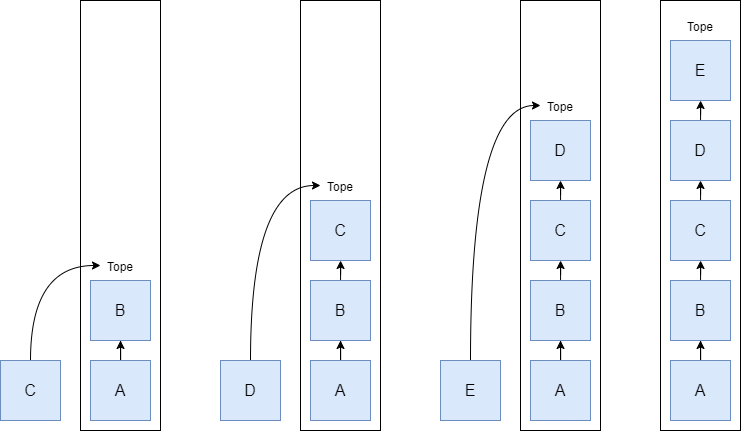
\includegraphics[width=0.8\textwidth]{pila_apilado.png}
\caption{\label{fig:seq01}Apilado en pila.}
\end{figure}


\begin{figure}[H]
\centering
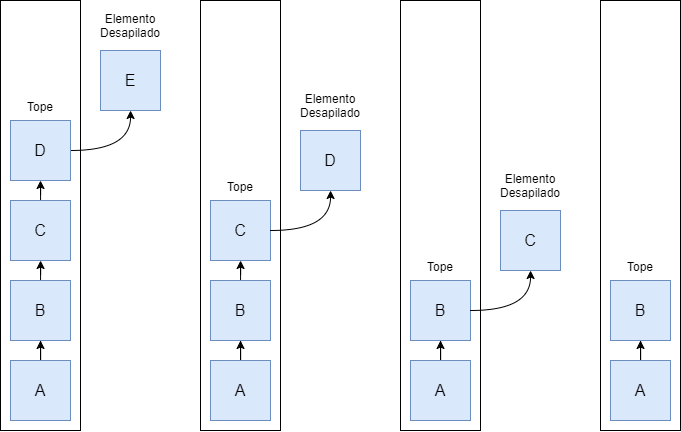
\includegraphics[width=0.8\textwidth]{pila_desapilado.png}
\caption{\label{fig:seq02}Desapilado en pila.}
\end{figure}


\begin{figure}[H]
\centering
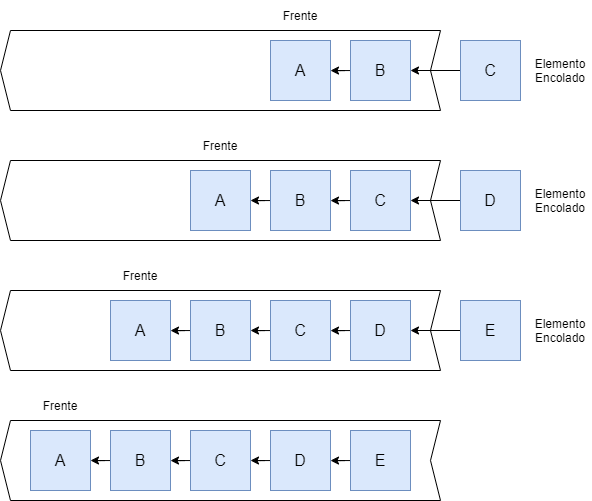
\includegraphics[width=0.8\textwidth]{cola_encolado.png}
\caption{\label{fig:seq03}Encolado en cola.}
\end{figure}


\begin{figure}[H]
\centering
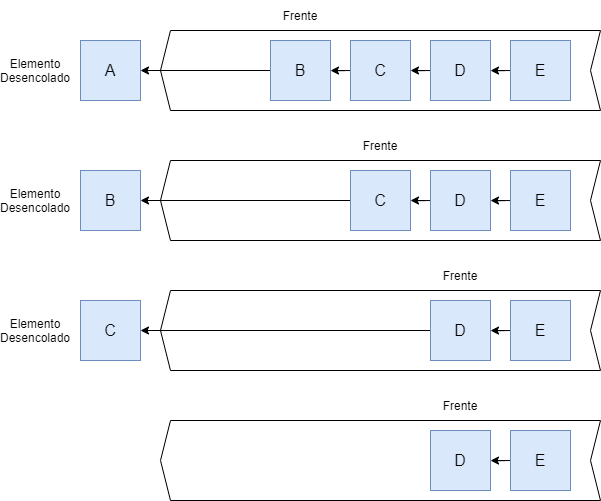
\includegraphics[width=0.8\textwidth]{cola_desencolado.png}
\caption{\label{fig:seq04}Desencolado en cola.}
\end{figure}


\begin{figure}[H]
\centering
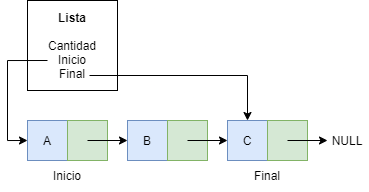
\includegraphics[width=0.8\textwidth]{lista_general.png}
\caption{\label{fig:seq05}Implementación de lista enlazada.}
\end{figure}


\begin{figure}[H]
\centering
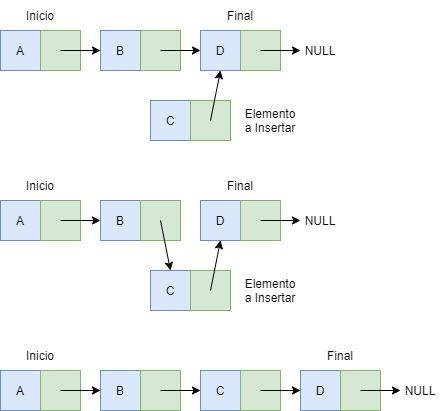
\includegraphics[width=0.8\textwidth]{lista_insercion.png}
\caption{\label{fig:seq06}Insertado en lista.}
\end{figure}


\begin{figure}[H]
\centering
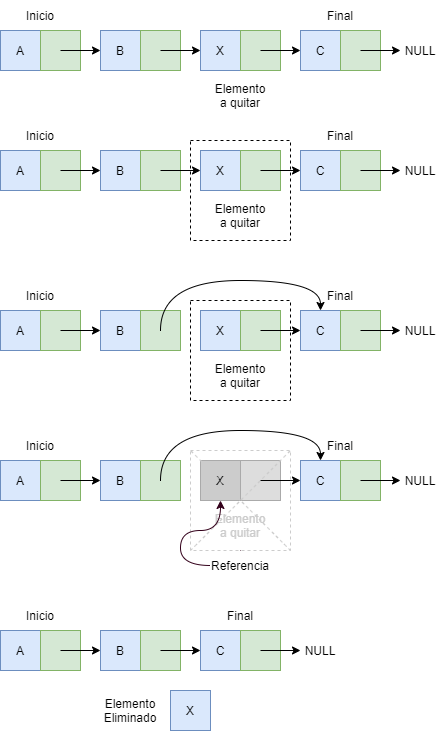
\includegraphics[width=0.8\textwidth]{lista_quitar.png}
\caption{\label{fig:seq07}Eliminación en lista.}
\end{figure}


\end{document}
